\documentclass[]{article}
\usepackage{blindtext}
\usepackage[T1]{fontenc}
\usepackage[utf8]{inputenc}
\usepackage{graphicx}
\usepackage[section]{placeins}


\title{%
	e-Yantra Ideas Competition 2019-20
	\\
	}
\author{
\\
\textbf{Project Name - Automatic Traffic Signal Timer}}

\date{\ }

\begin{document}

\maketitle



\section*{Introduction/Motivation:}
We have monitored these days that we have to wait on red lights even when there is no vehicle on the other side to cross the road. This is wastage of time in a city like Delhi / NCR to wait for approx 1 minute and it burns lakhs of litres of diesel every day.
\\
So we are introducing the automatic traffic signal timer that will automatically switch the traffic signal light if there is less or no vehicle on the road. This will work as follows:-
\\
We will use existing installed cameras on traffic lights or we can install new cameras which will monitor the vehicle density on road and if there is no or less vehicle to cross over the road and the traffic signal is green then it will automatically switch to red signal and provide green signal to other side of the road.

\section*{Literature Survey / Prior Network}
Traffic management is poor in our country and rarely considered as a major issue. There are few methods that are currently being in use like Automated number plate recognition, global shutter support and smart signal.
\\
A report from CRRI claims that the amount of fuel burnt in just idling of vehicle at traffic signals is about 39,806 kg and it produced 115 tonnes of carbon dioxide. These figures are just collected from eight traffic junction of Delhi and if calculate the whole figure from all busy crossroads of Delhi then the number will be much bigger than this.

\section*{Hardware Requirement - }
1. Raspberry pi.
\\
2. High resolution cameras.
\\
3. RF/UHF Transmitter and Receiver.

\section*{Software Requirement - }
1. Arduino IDE.
\\
2. Server.
\\
3. Eclipse.
\\
4. MATLAB / OPEN CV


\section*{Implementation}
The implementation of automatic traffic timer controller can be done in the following manner:
\\
1) First of all it captures the image of all the four sides of road.
\\
2) Using Open CV commands we can process that image to calculate the traffic density on the road.
\\
3) Compare the images i.e. their traffic density.
\\
4) The side of square road which is highly congested will be given priority for green signal.
\\
\\
The camera will be mounted on all the four traffic signal of square road. These camera will capture image of traffic in equal interval of time. These images get processed and thus used to calculate density on roads. 
\\
This calculation of density will go to Arduino board in which we had done our coding of arranging image according to their densities and then allow time stamp of traffic signal to get reduced if required.

\begin{figure}[!htb]
\begin{center}
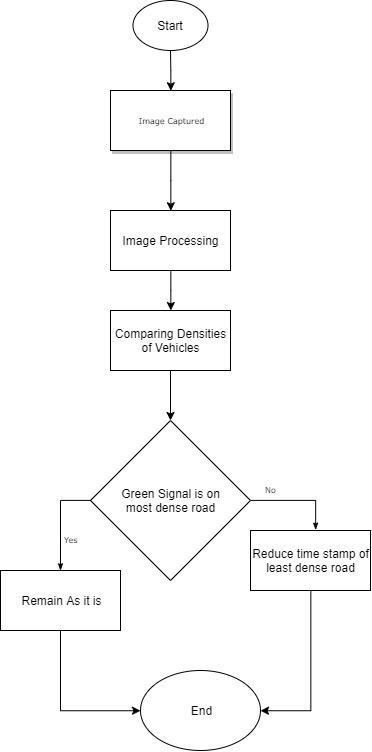
\includegraphics[scale=.65]{1.jpg}
\caption{Flow Diagram Of Automatic Traffic Signal Timer}
\end{center}
\end{figure}

\begin{figure}[!htb]
\begin{center}
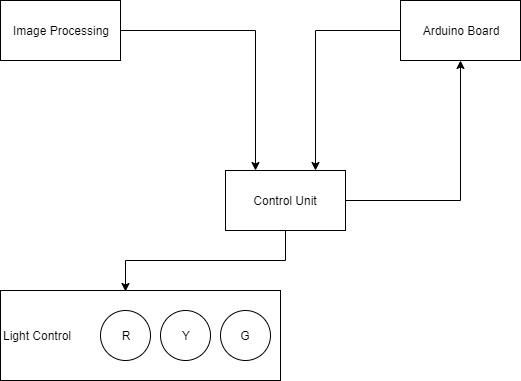
\includegraphics[scale=.70]{2.jpg}
\caption{Flow Diagram Of Devices}
\end{center}
\end{figure}

\pagebreak

\section*{Feasibility}
This project is beneficial for the passenger to travel easily from a less dense traffic signal.


\subsection*{i-   Technical Feasibility}
Our project will require mostly easy to available hardware and open source software, so our project is technically feasible.


\subsection*{ii-  Economic Feasibility}
This project is economically feasible as the software and hardware we are using( except camera) are not so much costly. Further it will also save passenger's money by avoiding them of burning unnecessary fuel on traffic signal.

\subsection*{iii-  Operational Feasibility}
This project is easy to operate as camera will capture image which get processed to calculate density of vehicle and then according to priority of density time stamp of traffic light timer will change.

\section*{References}
1.	https://en.wikipedia.org/wiki/Smart traffic light
\\
2. https://en.wikipedia.org/wiki/Raspberry Pi
\\
3. http://www.iitk.ac.in/nerd/web/articles/adaptive-traffic-light-timer-control-atltc

\end{document}